\section{Agregando información}
Una vez tenemos un buen modelo con los datos proporcionados, nos interesa agregar nuevos datos de otras fuentes que podrían complementar, y mejorar aun más las métricas previamente vistas.

La \href{https://www.who.int/data/gho/data/themes/mortality-and-global-health-estimates}{WHO} provee características distintas a las utilizadas en la experimentación hasta el momento, por lo que fue seleccionada como fuente. Una de ellas es la tasa de homicidios por cada 100000 habitantes\footnote{https://www.who.int/data/gho/data/indicators/indicator-details/GHO/estimates-of-rates-of-homicides-per-100-000-population}.

Es interesante poder analizar el impacto que las muertes no naturales por homicidio traen sobre la expectativa de vida general, así que se eligió para agregar al modelo ya definido.

Antes de poder utilizar los datos se tuvo que aplicar un proceso de limpieza de los mismos. Se analizo las columnas que el dataset tenia y lo que nos interesa de la misma. Las columnas que utilizamos fueron:
\begin{itemize}
    \item Period, el año del que provienen los datos de la medición.
    \item Dim1ValueCode, una variable categórica de 3 posibles valores.MLE(Male),FMLE(Female) y BTSX(Both sex).
    \item Location, el país al que corresponden los datos de la medición.
    \item FactValueNumeric, el valor promedio para la taza de homicidios.
\end{itemize}

El resto de las columnas tenían valores que aportaban poco una vez seleccionamos FactValueNumeric como el valor a usar(FactValueNumericLow,FactValueNumericHigh,Value). Columnas que tenían todos sus campos nulos, o repetidos. Y algunas que decidimos descartar porque ya estaban en los datos que teníamos(ParentLocation).

La manera en la que se limpiaron los datos fue la siguiente. Inicialmente, se eliminaron los datos con Period inferior a 2015, pues nuestro dataset en uso tiene en cada columna los promedios de los valores de cada año entre 2015 y la actualidad. Luego, nos quedamos con los valores Dim1ValueCode BTSX, dado que los datos de nuestro dataset no segregan por genero, y vamos a tener que unificarlos.Después de realizar los filtros mencionados nos quedamos con las columnas Location y FactValueNumeric. Se realiza un promedio entre las filas con la misma Location(los distintos años de la medición para ese país) y finalmente, se une al dataset original utilizando Location del dataset nuevo junto con Country del dataset original.

\begin{figure}[H]
              \centering
              \begin{subfigure}{0.5\linewidth}
                \centering
                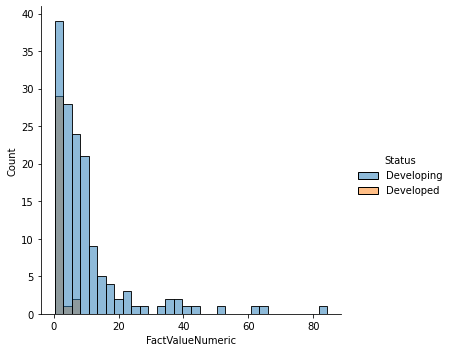
\includegraphics[width=\textwidth]{img/dist_homicides.png}
              \end{subfigure}
               \caption{Distribución de homicidios para países desarrollados y en vias de desarrollo.}
               \label{fig:dist_homicides}
        \end{figure}

En la figura \ref{fig:dist_homicides} podemos ver una distribución parecida a otras previamente vistas, como la figura \ref{fig: 4} para HIV/AIDS, solo que menos pronunciada en los primeros valores. Del mismo modo que la figura previamente mencionada, al separar entre Developing y Developed encontramos que la cantidad de suicidios para los países desarrollados es por mucho inferior a los no desarrollados, por lo que no aporta demasiado a este tipo de clasificación.
Como hipótesis respecto a esta característica se puede pensar que la tasa de homicidios va a tener algún tipo de influencia sobre la expectativa de vida, pues las muertes de causa no natural son un elemento categórico importante sobre las causas de muerte.

Para evaluarla, realizamos una ejecución de las métricas agregando a nuestro modelo mas completo la nueva característica.

Al ejecutar el predictor con la variable nueva se ve como el R2 ajustado empeora del 0.84873507 previo a 0.84787597, que, aun sin ser una disminución muy grande nos parecería indicar que no vale la pena agregarlo al predictor hasta este punto. Antes de descartar la característica decidimos aplicarle una función no lineal.

La función no lineal aplicada es logarítmica. Nuestra nueva característica mejora la predicción tanto para el R2 como el R2 ajustado, por lo que vale la pena conservarla en una nueva versión del mismo. El R2 pasa a ser de 0.8559576 y el ajustado de 0.85104706.

\begin{figure}[H]
              \centering
              \begin{subfigure}{0.5\linewidth}
                \centering
                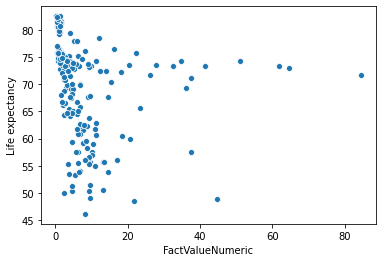
\includegraphics[width=\textwidth]{img/homicide_life_expectancy.png}
              \end{subfigure}
               \caption{Relación entre homicidios cada 1000 habitantes y expectativa de vida para un país.}
               \label{fig:life_expectancy_homicides}
        \end{figure}

Un posible motivo por el que nuestra característica responde mejor a una función logarítmica puede deberse a su relación con la expectativa de vida. En la figura \ref{fig:life_expectancy_homicides} podemos ver que  una expectativa de vida alta esta muy relacionada a una baja cantidad de homicidios, y al aumentar los mismos, la disminución de la expectativa de vida no es tan pronunciada.